% !TEX root = ./../tesis-usach.tex
% !TEX program = xelatex
% !BIB program = bibtex
\chapter{Multi-GPU}
\label{cap:multigpu}
La tarjeta Tesla K80 es una GPU que contiene dos tarjetas en una sola. Junto a ello, un sistema puede tener múltiples tarjetas GPU de alto cómputo. Por lo que se han querido aprovechar estas características para construir una solución que pueda ser usada tanto en una sola GPU como en múltiples, permitiendo así conseguir un mayor \textit{speedup}. A continuación se especifican las características de la solución para múltiples GPU.



\section{Comunicación Peer-to-Peer}
Una tarjeta puede comunicarse con la memoria de otra si es que la aplicación es ejecutada como un proceso de 64-bit y si la capacidad de cómputo de las tarjetas es 2.0 o más. Por ejemplo, una función que se ejecuta en GPU (\textit{kernel}) puede ejecutarse en una tarjeta y referenciar a un puntero cuya memoria haya sido almacenado en otra. Esto permite que la comunicación entre tarjetas sea más rápida debido a que si el acceso \textit{peer-to-peer} se habilita por medio de \texttt{cudaDeviceEnablePeerAccess()} ya no es necesario que los datos pasen por la memoria del sistema \citep{cuda}.
%Imagen Peer-to-Peer
Antes de utilizar la tecnología \textit{peer-to-peer} es necesario saber cuál es la topología del sistema para saber como los dispositivos PCI Express se conectan entre ellos y con CPU, esto es posible mediante el comando \texttt{nvidia-smi topo -m}. Por ejemplo, la topologia de Belka, sistema en donde se hacen las pruebas de este trabajo, puede verse en la Tabla \ref{tab:topology}.

\begin{table}[h!]
	\centering
	\begin{tabular}{@{}cccccccccc@{}}
		\toprule
		      & GPU 0 & GPU 1 & GPU 2 & GPU 3 & GPU 4 & GPU 5 & GPU 6 & GPU 7 & CPU Affinity \\ \midrule
		GPU 0 & X     & PIX   & PHB   & PHB   & SOC   & SOC   & SOC   & SOC   & 0-9          \\
		GPU 1 & PIX   & X     & PHB   & PHB   & SOC   & SOC   & SOC   & SOC   & 0-9          \\
		GPU 2 & PHB   & PHB   & X     & PIX   & SOC   & SOC   & SOC   & SOC   & 0-9          \\
		GPU 3 & PHB   & PHB   & PIX   & X     & SOC   & SOC   & SOC   & SOC   & 0-9          \\
		GPU 4 & SOC   & SOC   & SOC   & SOC   & X     & PIX   & PHB   & PHB   & 10-19        \\
		GPU 5 & SOC   & SOC   & SOC   & SOC   & PIX   & X     & PHB   & PHB   & 10-19        \\
		GPU 6 & SOC   & SOC   & SOC   & SOC   & PHB   & PHB   & X     & PIX   & 10-19        \\
		GPU 7 & SOC   & SOC   & SOC   & SOC   & PHB   & PHB   & PIX   & X     & 10-19        \\ \bottomrule
	\end{tabular}
	\caption{Topología de Belka}
	\label{tab:topology}
\end{table}

Las sigla PIX representa una comunicación a través de switch PCI Express interno, PHB representa la comunicación a través de un \textit{host bridge} PCI Express y finalmente SOC representa la comunicación a nivel de socket. Esto nos dice que hay 4 Tesla K80 conectadas al sistema (recordar que una Tesla K80 contiene dos tarjetas conectadas mediante un switch interno) pero que un par está separado de otro mediante un socket. Por lo tanto, solo es posible realizar comunicación P2P entre las GPU cero, uno, dos y tres; y las GPU, cuatro, cinco, seis, y siete.

\begin{figure}[h!]
	\centering
	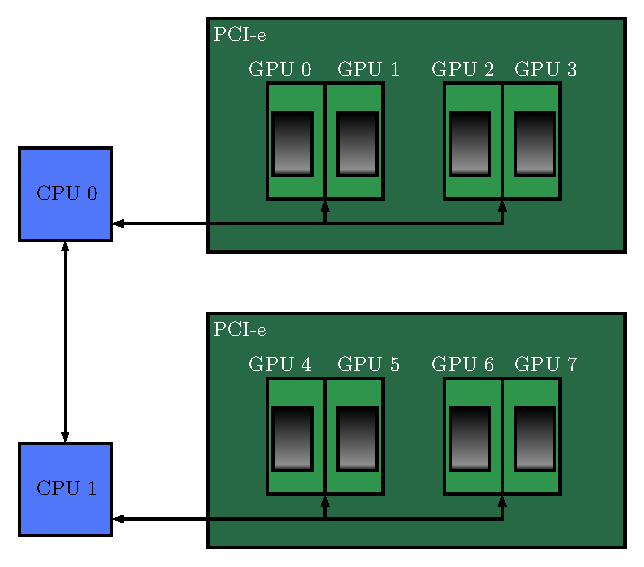
\includegraphics[scale=0.8]{./images/p2p.eps}
	\caption{Ilustración de la topología de Belka. Fuente: Elaboración propia}
	\label{fig:belkap2p}
\end{figure}

En la Figura \ref{fig:belkap2p} se aprecia que en Belka existen dos puertos PCI-Express con dos Tesla K80 conectadas a cada uno. Cada puerto PCI-Express se conecta con una CPU de 10 cores cada una. Con esta topología solo es posible realizar una conexión \textit{peer-to-peer} entre GPUs pertenecientes al mismo puerto.

\section{Direccionamiento Virtual Unificado}

Es posible que todos los dispositivos GPU y la CPU, utilicen un único espacio de memoria si todos los dispositivos tienen una capacidad de cómputo mayor o igual a 2.0. Como consecuencia, cuando se copia memoria a un dispositivo que está usando un espacio de direcciones unificado el parámetro \texttt{cudaMemcpyKind} de \texttt{cudaMemcpy()}, puede ser seteado a \texttt{cudaMemcpyDefault} para que CUDA automáticamente determine donde se encuentra almacenada la memoria de los punteros \citep{cuda}.

Cualquier puntero de memoria en algún dispositivo puede ser creado por un \textit{thread} del host y puede ser directamente referenciado dentro del mismo proceso. Sin embargo, esto no es posible fuera del proceso, por lo tanto, no se puede referenciar directamente a un puntero de memoria que pertenezca a un proceso distinto. Es por ello que para paralelizar el uso de múltiples GPU, y debido a que los threads que se crean pertenecen al mismo proceso se ha optado por usar OpenMP \citep{cuda}.

\section{OpenMP}

Para acelerar el cálculo de $\chi^{2}$ y $\nabla \chi^{2}$ es necesario que el uso de las múltiples tarjetas sea de forma paralela. Para ello, hay que tener en cuenta que cualquier thread del proceso ejecutado puede ejecutar la instrucción \texttt{cudaSetDevice(x)} que cambia la GPU con la cual se trabajará, por lo que los \textit{kernels} que sean ejecutados desde ese punto en adelante serán ejecutados en la GPU $x$. Es posible usar esta instrucción de forma paralela y así hacer que cada thread invoque \textit{kernels} en una GPU distinta y de forma concurrente. Por ejemplo, supongamos que se trabaja con el set de datos de HLTau en banda seis. Este set de datos tiene cuatro \textit{spectral windows} y cuatro canales por cada una de éstas. Además el usuario puede ingresar como argumento el número de GPUs que desea utilizar, siendo el número total de canales la máxima cantidad de GPUs a utilizar. Asimismo, se usa la claúsula \texttt{\# pragma omp parallel for schedule(static,1)} de OpenMP para recorrer los canales de todas las \textit{spectral windows} de forma paralela planificando las hebras de forma Round Robin como se muestra en la Figura \ref{fig:openmp}.

\begin{figure}[h!]
	\centering
	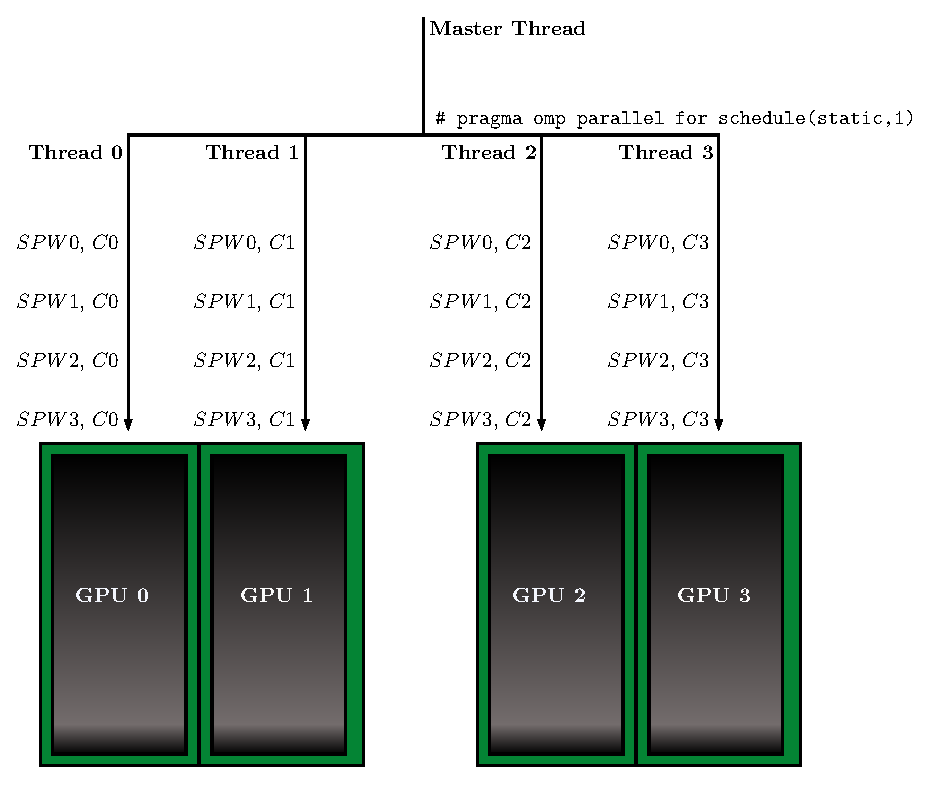
\includegraphics[scale=0.8]{./images/openmp.eps}
	\caption{Uso de OpenMP en múltiples GPUs. Fuente: Elaboración propia}
	\label{fig:openmp}
\end{figure}

Debido a que tanto para el cálculo de $\chi^{2}$ y $\nabla \chi^{2}$ se necesitan sumar los valores tanto de la función objetivo como del gradiente calculados en cada GPU respectivamente, se hace necesario crear  secciones críticas, es decir, regiones en donde sólo un thread del \textit{host} pueda ingresar a la vez, con el fin de que no existan condiciones de carrera entre ellos. Para ello, se utiliza la claúsula \texttt{\# pragma omp critical} de OpenMP. De esta forma se asegura que los cálculos de $\chi^{2}$ y $\nabla \chi^{2}$ en múltiples frecuencias sean los correctos. Cabe destacar que para el cálculo de $\nabla \chi^{2}$ en estos casos, se necesita un \textit{kernel} ubicado en la sección crítica que sume los valores de todos los dispositivos GPU.


\renewcommand{\algorithmicdo}{\textbf{do in parallel}}

\begin{algorithm}
	\begin{algorithmic}[1]
    \STATE{$\chi^{2} = 0$}
    \FOR{$i=0$ \TO TOTAL CHANNELS}
    \STATE{Compute $\chi^{2}_{i}$}
    \STATE{\textbf{BEGIN CRITICAL SECTION}}
    \STATE{$\chi^{2} = \chi^{2} + \chi^{2}_{i}$}
    \STATE{\textbf{END CRITICAL SECTION}}
    \ENDFOR
	\end{algorithmic}
	\caption{Cálculo de $\chi^{2}$ en paralelo}
	\label{alg:chi2openmp}
\end{algorithm}

\begin{algorithm}
	\begin{algorithmic}[1]
    \STATE{$\nabla \chi^{2} = 0$}
    \FOR{$i=0$ \TO TOTAL CHANNELS}
    \STATE{Compute $\nabla \chi^{2}_{i}$}
    \STATE{\textbf{BEGIN CRITICAL SECTION}}
    \STATE{$\nabla \chi^{2} = \nabla \chi^{2} + \nabla \chi^{2}_{i}$}
    \STATE{\textbf{END CRITICAL SECTION}}
    \ENDFOR
	\end{algorithmic}
	\caption{Cálculo de $\nabla \chi^{2}$ en paralelo}
	\label{alg:chi2openmp}
\end{algorithm}

\renewcommand{\algorithmicdo}{\textbf{do}}
